\documentclass[../main.tex]{subfiles}

\begin{document}
%%%%%%%%%%%%%%%%%%%%%%%%%%%%%%%%%%%%%%%%%%%%%
%                                           %
% PoMehrdimensionale Differentialrechnung I %
%                                           %
%%%%%%%%%%%%%%%%%%%%%%%%%%%%%%%%%%%%%%%%%%%%%
\chapter{SW13 Mehrdimensionale Differentialrechnung I}
\section{Multivariate Funktionen}
$f(x,y)=x+y$, wobei $\mathbb{R}^2\to\mathbb{R}$ ($\mathbb{R}^2$ weil zwei Argumente, $(x,y)$) \\

\section{Konturlinie}
Um Kontur- oder Niveaulinien für irgend ein Niveau $c$ zu zeichnen, muss man die 
Gleichung $f(x,y)=c$ nach $(x,y)$ auflösen.

\subsection{Beispiel}
$f(x,y)=x^2-y^2$ \\ [7pt]
Konturlinie: $f(x,y)=c=$ const \\ [7pt]
$x^2-y^2=c$ \\ [7pt]
$y=\pm\sqrt[]{x^2-c}$ \\ [7pt]
$x=\pm\sqrt[]{y^2+c} $

\section{Partielle Ableitung}
\begin{minipage}{0.45\textwidth}
    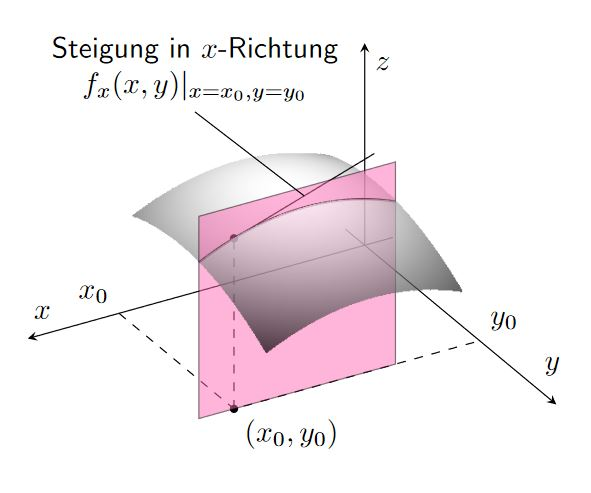
\includegraphics[width=50mm,scale=0.5]{partielle_ableitung_01}
\end{minipage} \hfill
\begin{minipage}{0.5\textwidth}
    Sei $f$ eine reellwertige Funktion von zwei Variablen. Wir betrachten die Ebene $y=y_0$ für eine Konstante 
    $y_0$. Dann hängt die Funktion \\ [7pt]
    $g(x)=f(x,y_0)$ \\ [7pt]
    nur noch von der einen Varbialen $x$ ab. Diese Funktion können wir mit den bereits bekannten Methoden nach
    $x$ ableiten. Das Resultat ist nichts anderes, als die partielle Ableitung von $f$ nach $x$. \\
\end{minipage}
$g'(x)=f_x(x,y_0)=\frac{\partial f(x,y)}{\partial x}|_{x,y=y_0}$ \\ [7pt]
an der Stelle $(x,y=y_0)$. \\
Hier bezeichnen $f_x$, oder $\frac{\partial f(x,y)}{\partial x}$, die partielle Ableitung von $f$ nach der Variablen $x$. \\

\begin{minipage}{0.45\textwidth}
    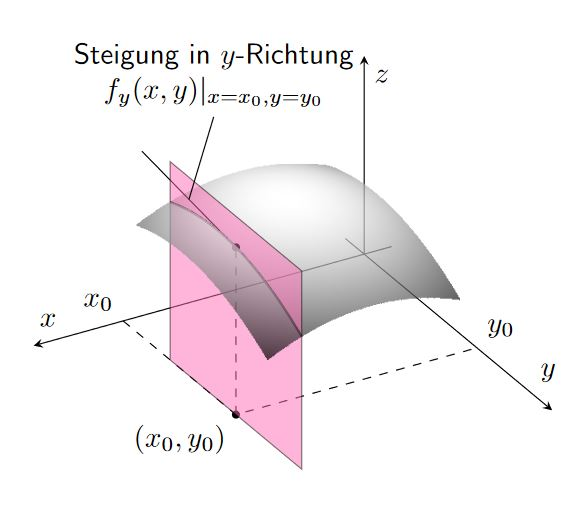
\includegraphics[width=50mm,scale=0.5]{partielle_ableitung_02}
\end{minipage} \hfill
\begin{minipage}{0.5\textwidth}
    Analog können wir $x=x_0$ fixieren und erhalten eine Funktion, die nur noch von $y$ abhängt: \\ [7pt]
    $h(y)=f(x_0,y)$ \\ [7pt]
    Die gewöhnliche Ableitung von $h$ nach $y$ ist dann nichts anderes, als die partielle Ableitung von $f$ nach $y$ 
\end{minipage}
$h'(y)=f_y(x_0,y)=\frac{\partial f(x,y)}{\partial x}|_{x=x_0,y}$ \\ [7pt]
an der Stelle $(x=x_0,y)$. \\
Wieder bezeichnen $f_y$, oder $\frac{\partial f(x,y)}{\partial x}$, die partielle Ableitung von $f$ nach der Variablen $y$.

\subsection{Definition}
Die partiellen Ableitungen von $f$ nach $x$ und $y$ an der Stelle $(x_0,y_0)$ sind nach dem oben Gesagten
wie folgt definiert: \\ [7pt]
$\frac{\partial f}{\partial x}|_{(x_0,y_0)}=f_x(x_0,y_0)=$ \\ [7pt]
Änderungsrate von $f$ bezüglich $x$ in $(x_0,y_0)$ \\ [7pt]
$ =\lim\limits_{h\to 0}\frac{f(x_0+h,y_0)-f(x_0,y_0)}{h}$ \\ [7pt]
$\frac{\partial f}{\partial y}|_{(x_0,y_0)}=f_y(x_0,y_0)=$ \\ [7pt]
Änderungsrate von $f$ bezüglich $y$ in $(x_0,y_0)$ \\ [7pt]
$ =\lim\limits_{h\to 0}\frac{f(x_0,y_0+h)-f(x_0,y_0)}{h}$

\subsection{Beispiel 1}
Sei $f(x,y)=\frac{x^2}{y+1}$. Gesucht $f_x(3,2)$ \\ [7pt]
$\frac{\partial f}{\partial x}=\frac{1}{y+1}\cdot 2x = \frac{2x}{y+1}$ \\ [7pt]
$\frac{\partial f}{\partial x}|_{(3,2)} = \frac{2\cdot 3}{2+1}=2$

\subsection{Beispiel 2}
$f(x,y)=(3xy+2x)^5$ \\ [7pt]
$\frac{\partial f}{\partial x}=5(3xy+2x)^4\cdot (3y+2)$ (nach x abgeleitet)\\ [7pt]
$\frac{\partial f}{\partial y}=5(3xy+2x)^4\cdot (3x)$ (nach y abgeleitet)

\subsection{Beispiel 3}
$f(x,y)=e^{x+3y}\sin(x,y)$ \\ [7pt]
$\frac{\partial f}{\partial x} = e^{x+3y}\cdot 1\cdot \sin(x,y) + e^{x+3y}\cdot \cos(x,y) \cdot y$
$=e^{x+3y}(\sin(x,y)+y\cos(x,y))$ \\
$\frac{\partial f}{\partial y}= e^{x+3y}\cdot 3\cdot \sin(x,y) + e^{x+3y}\cdot \cos(x,y) \cdot x$
$=e^{x+3y}(3\sin(x,y)+x\cos(x,y))$ 

\section{Definition - Der Gradient}
Sei $f$ eine reellwertige Funktion (ein Skalar) welche von zwei Variablen $x$ und $y$ abhängt. \\
Dann ist der Gradient von $f$ derjenige Vektor, dessen Komponenten die partiellen Ableitungen 
von $f$ nach den einzelnen Variablen sind, dh: \\ [7pt]
$\nabla f(\chi)=\begin{bmatrix}f_x(\chi) \\f_y(\chi)\end{bmatrix}$ oder ein bisschen ausführlicher
$\nabla f(x,y)=\begin{bmatrix}f_x(x,y) \\f_y(x,y)\end{bmatrix}$

\subsection{Beispiel 1}
Gesucht ist der Gradient von $f(x,y)=x+e^y$. Wie lautet der Gradient an der Stelle $(1,1)$. \\ [7pt]
$f_x(x,y)=\frac{\partial f}{\partial x}=1$ \\ [7pt]
$f_y(x,y)=\frac{\partial f}{\partial y}=e^y$ \\ [7pt]
$\nabla f(x,y)=\begin{bmatrix}f_x(x,y) \\f_y(x,y)\end{bmatrix} = \begin{bmatrix}1 \\e^y\end{bmatrix}$ \\ [7pt]
$\nabla f(1,1)=\nabla f|_{(1,1)}=\begin{bmatrix}1 \\e\end{bmatrix}$

\subsection{Beispiel 2}
Gesucht ist der Gradient von $f(x,y)=3x^2y$ für einen beliebigen Punkt. Wie lautet der Gradient an der Stelle $(1,1)$. \\ [7pt]
$f_x(x,y)=\frac{\partial f}{\partial x}=6xy$ \\ [7pt]
$f_y(x,y)=\frac{\partial f}{\partial y}=3x^2$ \\ [7pt]
$\nabla (x,y)=\begin{bmatrix}6xy \\3x^2\end{bmatrix}$ \\ [7pt]
$\nabla (1,1)=\begin{bmatrix}6 \\3\end{bmatrix}$ \\ [7pt]
$\nabla (0,0)=\begin{bmatrix}0 \\0\end{bmatrix}$

\subsection{Eigenschaften des Gradienten}
Ist $f$ eine anständige Funktion, dh insbesondere im Punkt $(x_0,y_0)$ differenzierbar mit dem 
Gradienten $\nabla f(x_0,y_0)\neq 0$, dann ist: \\
\begin{itemize}
    \item die Richtung des Gradienten $\nabla f(x_0,y_0)\neq 0$
    \begin{itemize}
        \item senkrecht (orthogonal) zu den Konturlinien von $f$ durch $(x_0,y_0)$, dh den Kurven mit $f(x_0,y_0)=f(x,y)$
        \item in Richtung der maximalen Zunahme von $f$
    \end{itemize}
    \item der Betrag des Gradienten $||\nabla f(x_0,y_0)||$ ist
    \begin{itemize}
        \item ist gleich der maximalen Änderungsrate von $f$ in diesem Punkt
        \item ist gross, wenn die Konturlinien nahe beieinander sind und klein, wenn sie weit auseinander liegen.
    \end{itemize}
\end{itemize}

\section{Richtungsableitung}
\begin{minipage}{0.45\textwidth}
    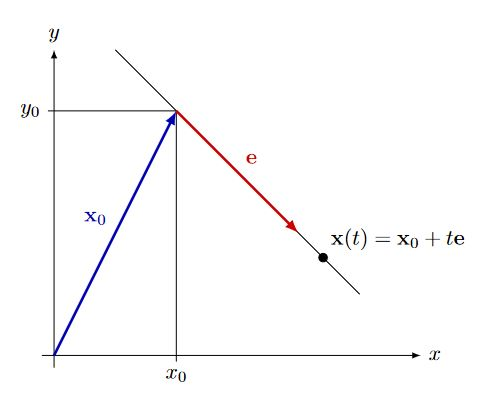
\includegraphics[width=50mm,scale=0.5]{richtungsableitung}
\end{minipage} \hfill
\begin{minipage}{0.5\textwidth}
    Die Änderungsrate wird Richtungsableitung von $f$ im Punkt $x_0$ in 
    Richtung von $e$ genannt und bezeichnet mit: \\ [7pt]
    $D_ef(x_0)=\lim\limits_{t\to 0+}\frac{f(x_0+te)-f(x_0)}{t}$
\end{minipage}

\subsection{Beispiel mit Richtungsvektor}
Berechne die Richtungsableitung von $f(x,y)=x+y$ (Ebene) im Punkt $x_0=[0,0]^T$ in Richtung
des Einheitsvektors $e=[\cos \psi, \sin \psi]^T$. Ist $e$ ein Einheitsvektor? \\
$f(x,y)=x+y$ \\ [7pt]
$P(0/0)$ \\ [7pt]
$e=\begin{pmatrix}\cos \psi \\\sin \psi\end{pmatrix}$ \\ [7pt]
$||e||$ bedeutet Länge von $e$ \\ [7pt]
$||e||^2=\cos^2\psi + \sin^2\psi=1$ \\ [7pt]
$||e||=1$ Vektor $e$ ist Einheitsvektor, weil länge $=1$\\ [7pt]
Ableitung von f im Punkt $P$ mit Richtung $e$: \\ [7pt]
$\textbf{f(p+te)}=f\left(\begin{pmatrix}0\\0\end{pmatrix} + t\begin{pmatrix}\cos \psi \\\sin \psi\end{pmatrix}\right)$
$=f\left(\begin{pmatrix}t\cos \psi \\t\sin \psi\end{pmatrix}\right)$
$f(t\cos\psi,t\sin\psi) = t\cos\psi + t\sin\psi = t(\cos\psi + \sin\psi) $ \\ [7pt]
$\textbf{f(p)}=f\left(\begin{pmatrix}0\\0\end{pmatrix}\right)=f(0,0)=0+0=0$  \\ [7pt]
$D_ef(0,0)=\lim\limits_{t \to 0}\frac{f(p+te)-f(p)}{t}$ 
$=\lim\limits_{t \to 0}\frac{t(\cos\psi + \sin\psi)}{t}=\cos\psi + \sin\psi$

\subsection{Beispiel ohne Richtungsvektor}
\textbf{Für einfachere Berechnung siehe \hyperref[sec:Richtungsableitung_Gradient]{\ref{sec:Richtungsableitung_Gradient} \nameref{sec:Richtungsableitung_Gradient}}}
Bestimme die Richtungsableitung von $f(x,y,z)=2x^2+3y^3+z^2$ in $x_0=[2,1,3]^T$ in Richtung von
$a=[1,0,-2]^T$. Beachte, $a$ ist kein Richtungsvektor. \\ [7pt]
$f(x,y,z)=2x^2+3y^3+z^2$ \\ [7pt]
$P(2/1/3)$ \\ [7pt]
$|a|=\sqrt{1^2+0^2+(-2)^2}=\sqrt{1+4}=\sqrt{5}$ \\ [7pt]
$a_0=e=\frac{a}{|a|}=\frac{1}{\sqrt{5}}\cdot\begin{pmatrix}1\\0\\-2\end{pmatrix}$ 
$=\begin{pmatrix}\frac{1}{\sqrt{5}}\\0\\\frac{-2}{\sqrt{5}}\end{pmatrix} $\\ [7pt]
$\textbf{f(p+te)}=f\left(\begin{pmatrix}2\\1\\3\end{pmatrix}+t\begin{pmatrix}\frac{1}{\sqrt{5}}\\0\\\frac{-2}{\sqrt{5}}\end{pmatrix}\right)$
$=f\left(\begin{pmatrix}2+\frac{t}{\sqrt{5}}\\1\\3-\frac{2t}{\sqrt{5}}\end{pmatrix}\right)$ 
$f(2+\frac{t}{\sqrt{5}},1,3-\frac{2t}{\sqrt{5}})$ \\ [7pt]
$x(t)=2+\frac{t}{\sqrt{5}}$ \\ [7pt]
$y(t)=1$ \\ [7pt]
$z(t)=3-\frac{2t}{\sqrt{5}}$ \\ [7pt]
$f(t) = 2(x(t))^2+3(y(t))^3+(z(t))^2$
$=2(2+\frac{t}{\sqrt{5}})^2+3(1)^3+(3-\frac{2t}{\sqrt{5}})^2 = \textbf{f(p + te)}$ \\
$D_ef(0,0)=\lim\limits_{t \to 0}\frac{f(p+te)-f(p)}{t}=...=-\frac{4}{\sqrt{5}}$ \\ [7pt]
Falls wir uns vom Punkt $p$ in Richtung des Vektors $a$ um eine Einheit bewegen, nimmt die
Funktion um $-\frac{4}{\sqrt{5}}$ ab.

\section{Richtungsableitung und Gradient}
\label{sec:Richtungsableitung_Gradient}
Für eine anständige (sprich differenzierbare) Funktion kann die Richtungsableitung von $f$
im Punkt $p$ in Richtung des Einheitsvektors $e$ mit Hilfe des Gradienten bestimmt werden: \\ [7pt]
$D_ef(p)=\nabla f(p)\cdot e=|\nabla f(p)|\cos\phi$

\subsection{Beispiel}
$f(x,y,z)=2x^2+3y^3+z^2$ \\ [7pt]
$P(2/1/3)$ \\ [7pt]
$|a|=\sqrt{1^2+0^2+(-2)^2}=\sqrt{1+4}=\sqrt{5}$ \\ [7pt]
$e=\frac{a}{|a|}=\frac{1}{\sqrt{5}}\cdot\begin{pmatrix}1\\0\\-2\end{pmatrix}$ \\
$\nabla f(x,y,z)=\begin{pmatrix}4x\\9y^2\\2z\end{pmatrix}$ \\ [7pt]
$\nabla f(2,1,3)=\begin{pmatrix}8\\9\\3\end{pmatrix}$ \\ [7pt]
$D_ef(2,1,3)=\nabla f(2,1,3)\cdot e = \begin{pmatrix}8\\9\\3\end{pmatrix} \cdot \frac{1}{\sqrt{5}}\cdot\begin{pmatrix}1\\0\\-2\end{pmatrix}$
$= \frac{1}{\sqrt{5}}\cdot((8\cdot1)+(9\cdot0)+(6\cdot-2))$ \\ [7pt]
$= \frac{1}{\sqrt{5}}\cdot(8+0-12)=\frac{-4}{\sqrt{5}}$

\end{document}